% TeX file "local_linear_regression"

% Research Module in Econometrics & Statistics 
% Prof. Dr. Liebl & Dr. Christopher Walsh
% Winter 2021/22, M.Sc. Economics, Bonn University
% Xingyu Tao, Xuan Li, Sven Jacobs


\section{Local linear regression} \label{sec:local_linear_regression}

We now first introduce local linear regression formally.
We then report the main results of the asymptotic analysis to compare both estimators.
A graphical approach illustrates the theoretical findings and builds intuition.

\subsection{Definition} \label{subsec:definition}

The Nadaraya-Watson estimator is also called a local constant estimator as it locally approximates the function $m$ as constant.
Hence, we obtain the estimator in \eqref{eq:nw} likewise from
\begin{equation}
	\hat{m}_{\NW}(x) = \argmin_{\beta_0} \sum_{i = 1}^{n} (Y_i - \beta_0)^2 K \left( \frac{X_i - x}{h} \right) \,.
\end{equation}
A natural extension is the weighted local fitting of a line with slope:
\begin{align}
	\hat{m}_{\LL}(x) &= \argmin_{\beta_0} \sum_{i = 1}^{n} (Y_i - \beta_0 - \beta_1(X_i - x))^2 K \left( \frac{X_i - x}{h} \right) \label{eq:ll} \\ 
	&= \sum_{i = 1}^{n} w(x, X_i, h) Y_i \,. \label{eq:linear_smoother}
\end{align}
We call $\hat{m}_{\LL}$ the local linear estimator.
From Equation~\eqref{eq:linear_smoother} we see that the estimator also belongs to the class of linear smoothers, i.e.\
it is a weighted average of the observed outcomes.
Since \eqref{eq:ll} is a standard weighted least squares problem, we obtain an explicit solution as (e.g.\ \cite[Section~5.2]{Wand_1995})
\begin{equation}
	\hat{m}_{\LL}(x) = \bm{e}_1^\top \left( \bm{X}_x^\top \bm{W}_x^{\vphantom{\top}} \bm{X}_x^{\vphantom{\top}} \right)^{-1} \bm{X}_x^\top \bm{W}_x^{\vphantom{\top}} \bm{Y} \,, 
\end{equation}
where invertibility of $\bm{X}_x^\top \bm{W}_x^{\vphantom{\top}} \bm{X}_x^{\vphantom{\top}}$ is assumed and 
\begin{equation}
	\bm{Y} = \begin{bmatrix} Y_1 \\ \vdots \\ Y_n \end{bmatrix},
	\bm{X}_x = \begin{bmatrix} 1 & X_1 - x \\ \vdots & \vdots \\ 1 & X_n - x  \end{bmatrix},
	\bm{W}_x = \diag \left\{ K \left( \frac{X_1 - x}{h} \right), \dots, K \left( \frac{X_n - x}{h} \right) \right\},
	\bm{e}_1 = \begin{bmatrix} 1 \\ 0 \\ \vdots \end{bmatrix} \,.
\end{equation}

If we apply the local linear estimator to the same data from Figure~\ref{fig:nw},
we achieve a much better estimation near the boundaries relative to the Nadaraya-Watson estimator.
This is depicted in Figure~\ref{fig:ll}.
To see how the bias is reduced, Figure~\ref{fig:ll_boundary} zooms in the estimation at the lower boundary $x = 0$.
Although half of the scaled kernel is not matched by any data, the estimated value is only slightly too high.
The reason is that the true curve can be well approximated by the fitted linear function on the interval $[0, 0.2]$. 
\begin{figure}
	\centering
	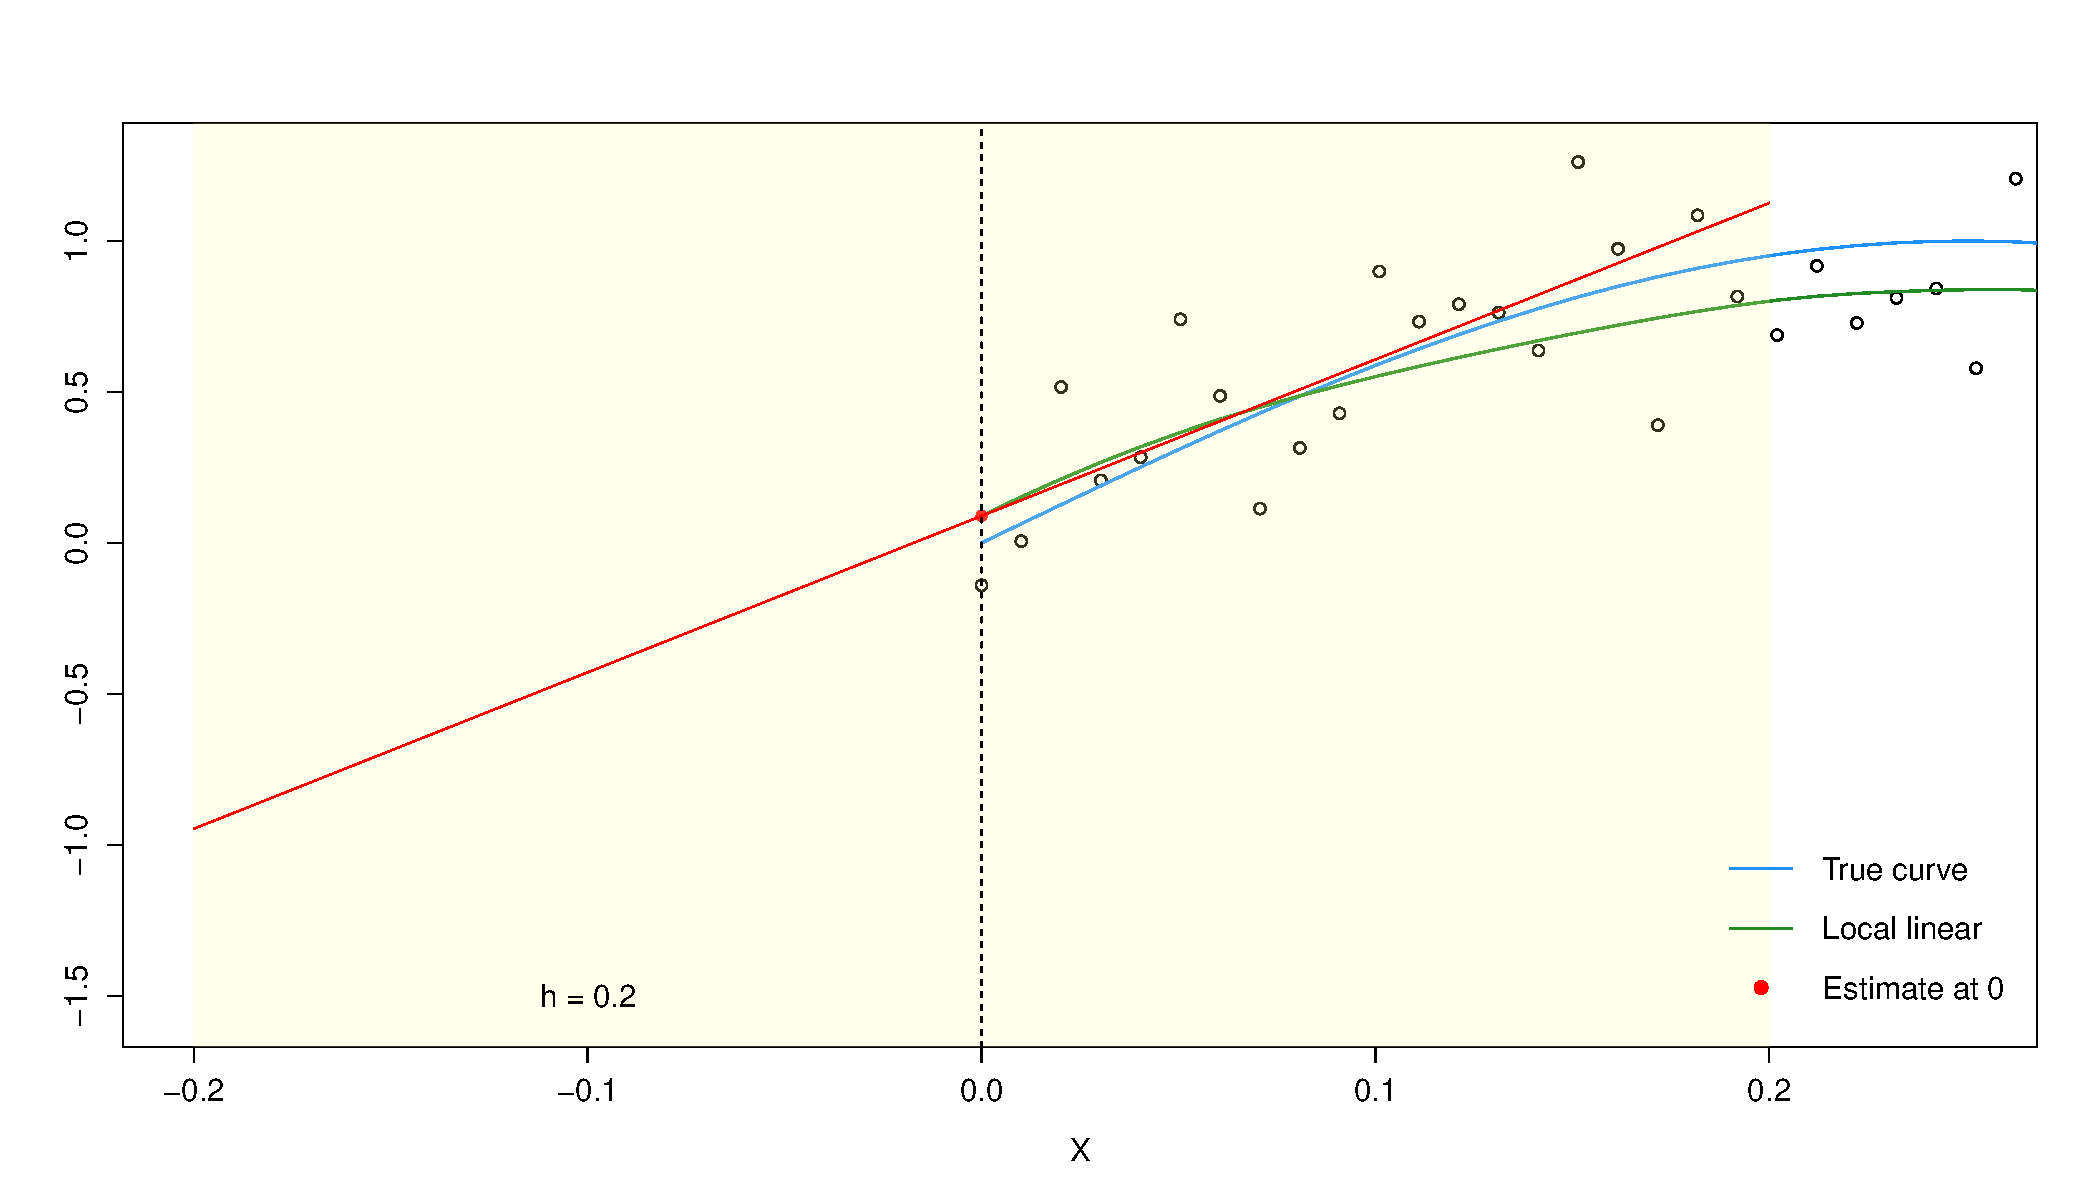
\includegraphics[trim=20 15 20 50, clip, width=0.75\textwidth]{figure_02.pdf}
	\caption{Illustration of the local linear estimate at the lower boundary $x = 0$.
			 Besides the point estimate also the locally fitted regression line is plotted.}
	\label{fig:ll_boundary}
\end{figure}

\begin{remark}
	Nadaraya-Watson ($p = 0$) and the local linear estimator ($p = 1$) are special cases of the local polynomial estimator,
	which locally fits a $p$-th degree polynomial to the data via least squares.
	To analyze the boundary correction provided by local polynomial regression, it suffices to look at the linear case.
\end{remark}

\subsection{Theoretical comparison} \label{subsec:theoretical_comparison}

The flexibility of nonparametric curve estimation makes a precise theoretical treatment for finite sample sizes complicated \parencite[15]{Härdle_1990}.
To gain the relevant insights into the performance of $\hat{m}_{\NW}$ and $\hat{m}_{\LL}$, we instead consider the asymptotic expressions,
i.e.\ the leading terms of bias and variance.
For the asymptotic analysis we rely on the following assumptions:
\begin{enumerate}[label=(A\arabic*), left=\parindent, itemsep=0pt]
	\item $m$ is twice continuously differentiable \label{A1}
	\item $f$ is continuously differentiable and $f(x)>0$
	\item $\sigma^2$ is continuous 
	\item $K$ is a symmetric and bounded pdf with $\kappa_2(K) \equiv \int u^2K(u) \diff u < \infty$ (finite variance) and $R(K) \equiv \int K(u)^2 \diff u < \infty$ (square integrability) \label{A4}
	\item $h \rightarrow 0, nh \rightarrow \infty$ as $n \rightarrow \infty$ \label{A5}
\end{enumerate}   
Assumption~\ref{A1} is a smoothness condition on the regression function needed for Taylor expansions.
We also assume certain smoothness of the design density $f$ and the conditional variance function $\sigma^2$.
The positive lower bound of $f$ is required because for the estimation the neighborhood of $x$ has to contain observations.
\ref{A4} states mild assumptions for the kernel function, which are satisfied for all kernels given in Table~\ref{tab:kernels}.
Lastly, to reduce bias the bandwidth $h$ has to get smaller yet the effective sample size $nh$ tends to infinity for the variance to vanish.

We start with the evaluation point $x$ being in the interior of the support of $f$.
Afterwards we move to the boundary.
The following theorem provides the core results for the estimation in the interior.
The proof for the Nadaraya-Watson estimator is presented in Appendix~\hyperref[appendix_1]{1}.
For the local linear estimator we refer the reader to \textcite[Section 3.7]{Fan_1996}.
\begin{theorem} \label{theorem_1}
	Let assumptions \ref{A1}--\ref{A5} be fulfilled and $x$ be in the interior of $\supp(f)$.
	Then, the conditional asymptotic bias is given by
	\begin{align}
		\ABias (\hat{m}_{\NW}(x) \,|\, \bm{X}) &= \frac{1}{2} \kappa_2(K) m''(x) h^2 + \kappa_2(K) \frac{m'(x)f'(x)}{f(x)} h^2 &=& \bigO(h^2) \,, \\
		\ABias (\hat{m}_{\LL}(x) \,|\, \bm{X}) &= \frac{1}{2} \kappa_2(K) m''(x) h^2 &=& \bigO(h^2) \,. \\
		\intertext{The conditional asymptotic variance is given by}
		\AVar (\hat{m}_{\NW}(x) \,|\, \bm{X}) &= \AVar (\hat{m}_{\LL}(x) \,|\, \bm{X}) = \frac{R(K) \sigma^2(x)}{f(x)} \frac{1}{nh} &=& \bigO\left( \frac{1}{nh} \right) \,.
	\end{align}
\end{theorem} 
Theorem~\ref{theorem_1} provides valuable insights into the properties of both estimators.
The asymptotic bias of $\hat{m}_{\LL}$ depends on the kernel constant $\kappa_2(K)$, the curvature of the unknown function $m$ and the squared bandwidth.
For a fixed bandwidth we obtain larger bias the curvier $m$.
Concavity leads to downward bias, convexity to upward bias.
This so-called smoothing bias (\enquote{trimming the hills and filling the valleys}) can also be seen in Figure~\ref{fig:ll}.
Overall, the order of $h^2$ means that for reduced bias in general a smaller bandwidth is required.
Looking next at the leading bias expression for the Nadaraya-Watson estimator, we notice the presence of a second term.
Due to its dependence on the design density the term is referred to as design bias.
Design bias is absent for uniform designs and more pronounced for stronger changes in $f$ and $m$.
Although the order of magnitude is the same, the interpretation is that $\hat{m}_{\LL}$ being design-adaptive \parencite{Fan_1992}
with simplified bias typically translates into reduced bias in practice \parencite[678]{Hansen_2022}.
Interestingly, the conditional asymptotic variance is the same for both estimators.
It is inversely proportional to the effective sample size, i.e.\ $\sim (nh)^{-1}$.

From Theorem~\ref{theorem_1} we can easily derive the asymptotically optimal local bandwidth minimizing the conditional asymptotic mean squared error (AMSE).
This yields $h_{\text{opt}}(x) \sim n^{-1/5}$ and $\AMSE_{\text{opt}}(x) \sim n^{-4/5}$.
An optimal global bandwidth is obtained as the minimizer of the density-weighted integrated AMSE (AMISE),
\begin{equation}
	h_{\text{opt}} \equiv \argmin_{h \,>\, 0} \int_{\supp(f)}^{} \AMSE(x) f(x) \diff x \,.
\end{equation} 
The solution for the Nadaraya-Watson and the local linear estimator, respectively, is given in the following theorem.
\begin{theorem} \label{theorem_2}
	The bandwidth minimizing the AMISE is given by
	\begin{align}
		h_{\textup{opt}}^{\LL}(n) &= \left\{ \frac{R(K) \int \sigma^2(x) \diff x}{\kappa_2(K)^2 \int (m''(x))^2 f(x) \diff x} \right\}^{1/5} \cdot n^{-1/5} \,, \\
		h_{\textup{opt}}^{\NW}(n) &= \left\{ \frac{R(K) \int \sigma^2(x) \diff x}{\kappa_2(K)^2 4 \mathlarger{\int} \left[ \frac{1}{2} m''(x) + \frac{m'(x) f'(x)}{f(x)} \right]^2 f(x) \diff x} \right\}^{1/5} \cdot n^{-1/5} \,.
	\end{align}
	With $h_{\textup{opt}} \sim n^{-1/5}$ it follows that $\AMISE_{\textup{opt}} \sim n^{-4/5}$. 
\end{theorem}     

In what follows we take $x$ to be exactly at the boundary, i.e.\ $x \in \{a, b\}$.
We draw on the same assumptions \ref{A1}--\ref{A5} as for the interior,
but now particularly require regarding \ref{A1} right-sided continuity at the lower boundary and left-sided continuity at the upper boundary.
In mathematical terms that is $\lim_{x \downarrow a} m''(x) = m''(a)$ and $\lim_{x \uparrow b} m''(x) = m''(b)$.
For the asymptotic theory of the local linear estimator at the boundary we define now truncated kernel moments, a projected kernel $\tilde{K}$ and its constants (see \cite[684]{Hansen_2022}):
\begin{align}
	\tilde{\kappa}_j(K) &\equiv \int_{0}^{\infty} u^jK(u) \diff u \,, \tilde{\tau}_j(K) \equiv \int_{0}^{\infty} u^jK(u)^2 \diff u \,, \\
	\tilde{K}(u) &\equiv \frac{\tilde{\kappa}_2 - \tilde{\kappa}_1 u}{\tilde{\kappa}_0^{\vphantom{2}} \tilde{\kappa}_2^{\vphantom{2}} - \tilde{\kappa}_1^2} K(u) \,, \\
	\tilde{\kappa}_2(\tilde{K}) &= \int_{0}^{\infty} u^2\tilde{K}(u) \diff u = \frac{\tilde{\kappa}_2^2 - \tilde{\kappa}_1^{\vphantom{2}}  \tilde{\kappa}_3^{\vphantom{2}}}{\tilde{\kappa}_0^{\vphantom{2}} \tilde{\kappa}_2^{\vphantom{2}} - \tilde{\kappa}_1^2} \,, \\
	\tilde{R}(\tilde{K}) &\equiv \int_{0}^{\infty} \tilde{K}(u)^2 \diff u = \frac{\tilde{\kappa}_2^2 \tilde{\tau}_0^{\vphantom{2}} - 2 \tilde{\kappa}_1^{\vphantom{2}} \tilde{\kappa}_2^{\vphantom{2}} \tilde{\tau}_1^{\vphantom{2}} + \tilde{\kappa}_1^2 \tilde{\tau}_2^{\vphantom{2}}}{(\tilde{\kappa}_0^{\vphantom{2}} \tilde{\kappa}_2^{\vphantom{2}} - \tilde{\kappa}_1^2)_{\vphantom{2}}^2} \,.
\end{align}

Theorem~\ref{theorem_3} reports the main results.
\begin{theorem} \label{theorem_3}
	Let assumptions \ref{A1}--\ref{A5} be fulfilled and $x \in \{a, b\}$. Then, the conditional asymptotic bias for $\hat{m}_{\NW}$ is given by
	\begin{align}
		\ABias (\hat{m}_{\NW}(a) \,|\, \bm{X}) &= 2 \int_{0}^{\infty} u K(u) \diff u \, m'(a) h &=& \bigO(h) \,, \\
		\ABias (\hat{m}_{\NW}(b) \,|\, \bm{X}) &= -2 \int_{0}^{\infty} u K(u) \diff u \, m'(b) h &=& \bigO(h) \,. \\
		\intertext{The conditional asymptotic bias and variance at $x = a$ for $\hat{m}_{\LL}$ is given by}
		\ABias (\hat{m}_{\LL}(a) \,|\, \bm{X}) &= \frac{1}{2} \tilde{\kappa}_2(\tilde{K}) m''(a) h^2 &=& \bigO(h^2) \,, \\
		\AVar (\hat{m}_{\LL}(a) \,|\, \bm{X}) &= \frac{\tilde{R}(\tilde{K}) \sigma^2(a)}{f(a)} \frac{1}{nh} &=& \bigO\left( \frac{1}{nh} \right) \,.
	\end{align}
\end{theorem}
For the local linear estimator see \textcite[Section 19.10]{Hansen_2022} and \textcite[Theorem 3.3]{Fan_1996}.
For the derivation of the asymptotic boundary bias of the Nadaraya-Watson estimator we follow the steps in the proof for interior points (Appendix~\hyperref[appendix_1]{1}).
However, since at the boundary half of the kernel is not contained in the support of $f$, the integral in \eqref{eq:appendix_1_03} is now over the region $[0, \infty)$.
As a consequence, the leading term is \eqref{eq:appendix_1_04}.

From Theorem~\ref{theorem_3} we see that the asymptotic bias and variance of $\hat{m}_{\LL}$ look very similar to the expressions from Theorem~\ref{theorem_1}.
Most importantly, the orders are unchanged.
What differs are the constants as they depend now on the projected kernel $\tilde{K}$.
In contrast, consulting the asymptotic bias of $\hat{m}_{\NW}$ at either boundary we notice the larger order of $h$ compared to $h^2$.
Because of this discrepancy between the bias order in the interior and at the boundary we say that the Nadaraya-Watson estimator exhibits a boundary bias problem.
The local linear estimator instead preserves the order.
Moreover, the equations show that if the regression function $m$ is positively sloped at the boundaries,
$\hat{m}_{\NW}$ will have upward bias at the lower boundary and downward bias at the upper boundary (see e.g.\ Figure~\ref{fig:nw}). 

For finite samples there is always a boundary region instead of just one or two boundary points.
If we assume that $\supp(K) = [-1, 1]$ and w.l.o.g.\ that $f$ is supported on the unit interval $[0, 1]$,
then the boundary region equals $[0, h) \cup (1-h, 1]$.
For $0 \leq \rho < 1$ we call $x = \rho h$ a left boundary point and $x = 1 - \rho h$ a right boundary point.
\textcite[Theorem~3.2]{Fan_1996} derived for an arbitrary boundary point qualitatively identical results as in Theorem~\ref{theorem_3},
including as a special case $x \in \{a, b\}$ being an exact boundary point.

It follows that the asymptotically optimal bandwidth near the boundary for the Nadaraya-Watson estimator is now $\bigO(n^{-1/3})$,
thus smaller bandwidths are required due to increased bias.
The optimal AMSE gets inflated to $\bigO(n^{-2/3})$ relative to $\bigO(n^{-4/5})$ in the interior.

So far our analysis has been of asymptotic nature.
However, we can show that the local linear estimator is exactly unbiased to first order, also in the boundary region.
To do so, we write the conditional expectation of either estimator as
\begin{align}
	\E [\hat{m}(x) \,|\, \bm{X}] &= \sum_{i = 1}^{n} w_i(x) m(X_i) \\
	&= m(x) \sum_{i = 1}^{n} w_i(x) + m'(x) \sum_{i = 1}^{n} w_i(x) (X_i - x) + R \,,
\end{align}
where in the second equality a Taylor expansion around $x$ is performed and $R$ contains higher-order terms.
The exact correction of the bias to first order by $\hat{m}_{\LL}$ follows immediately from the next theorem.
The proof is in Appendix~\hyperref[appendix_1]{1}. 
\begin{samepage}
	\begin{theorem} \label{theorem_4}
		Consider the estimation of the local linear estimator at some point $x$, i.e.\ $\hat{m}_{\LL}(x) = \sum_{i = 1}^{n} w_i(x) Y_i$.
		Then:
		\begin{align}
			\sum_{i = 1}^{n} w_i(x) &= 1 \,, \\
			\sum_{i = 1}^{n} w_i(x) (X_i - x) &= 0 \,.
		\end{align}
	\end{theorem}
\end{samepage}
If the true regression function is linear (as in Figure~\ref{fig:boundary_effects_linear}),
the local linear estimator will not have any estimation bias over the full design region.
For the Nadaraya-Watson estimator the term $\sum_{i = 1}^{n} w_i(x) (X_i - x)$ at the boundary is necessarily unequal to zero as the weights are nonnegative.

We briefly summarize the findings.
For the interior the order of the bias for both estimators is the same.
However, local linear regression has the favorable design-adaptivity property.
Near the boundary, the bias of the Nadaraya-Watson estimator is of larger order, whereas the local linear estimator preserves the order.
The latter is first-order unbiased.

\subsection{Graphical comparison}

By now we have shown mathematically that local linear regression fixes the boundary issue the Nadaraya-Watson estimator has.
To develop a deeper understanding for how the bias correction is achieved in practice, a graphical analysis is desirable.
An informative graphical device, based on the concept of an effective kernel, was proposed by \textcite{Hastie_1993}.
Since both estimators belong to the class of linear smoothers, they can be written as $\hat{m}(x)~=~\sum_{i = 1}^{n} w(x, X_i, h) Y_i$.
The effective kernel at an estimation point $x$ is then defined as the set of weights $\{w(x, X_i, h)\}_{i = 1}^n$,
i.e.\ the effective weights assigned to observations.
The idea is now to plot the effective kernel against the $X_i$'s.

\begin{figure}[t]
	\centering
	\begin{subfigure}{0.75\textwidth}
		\centering
		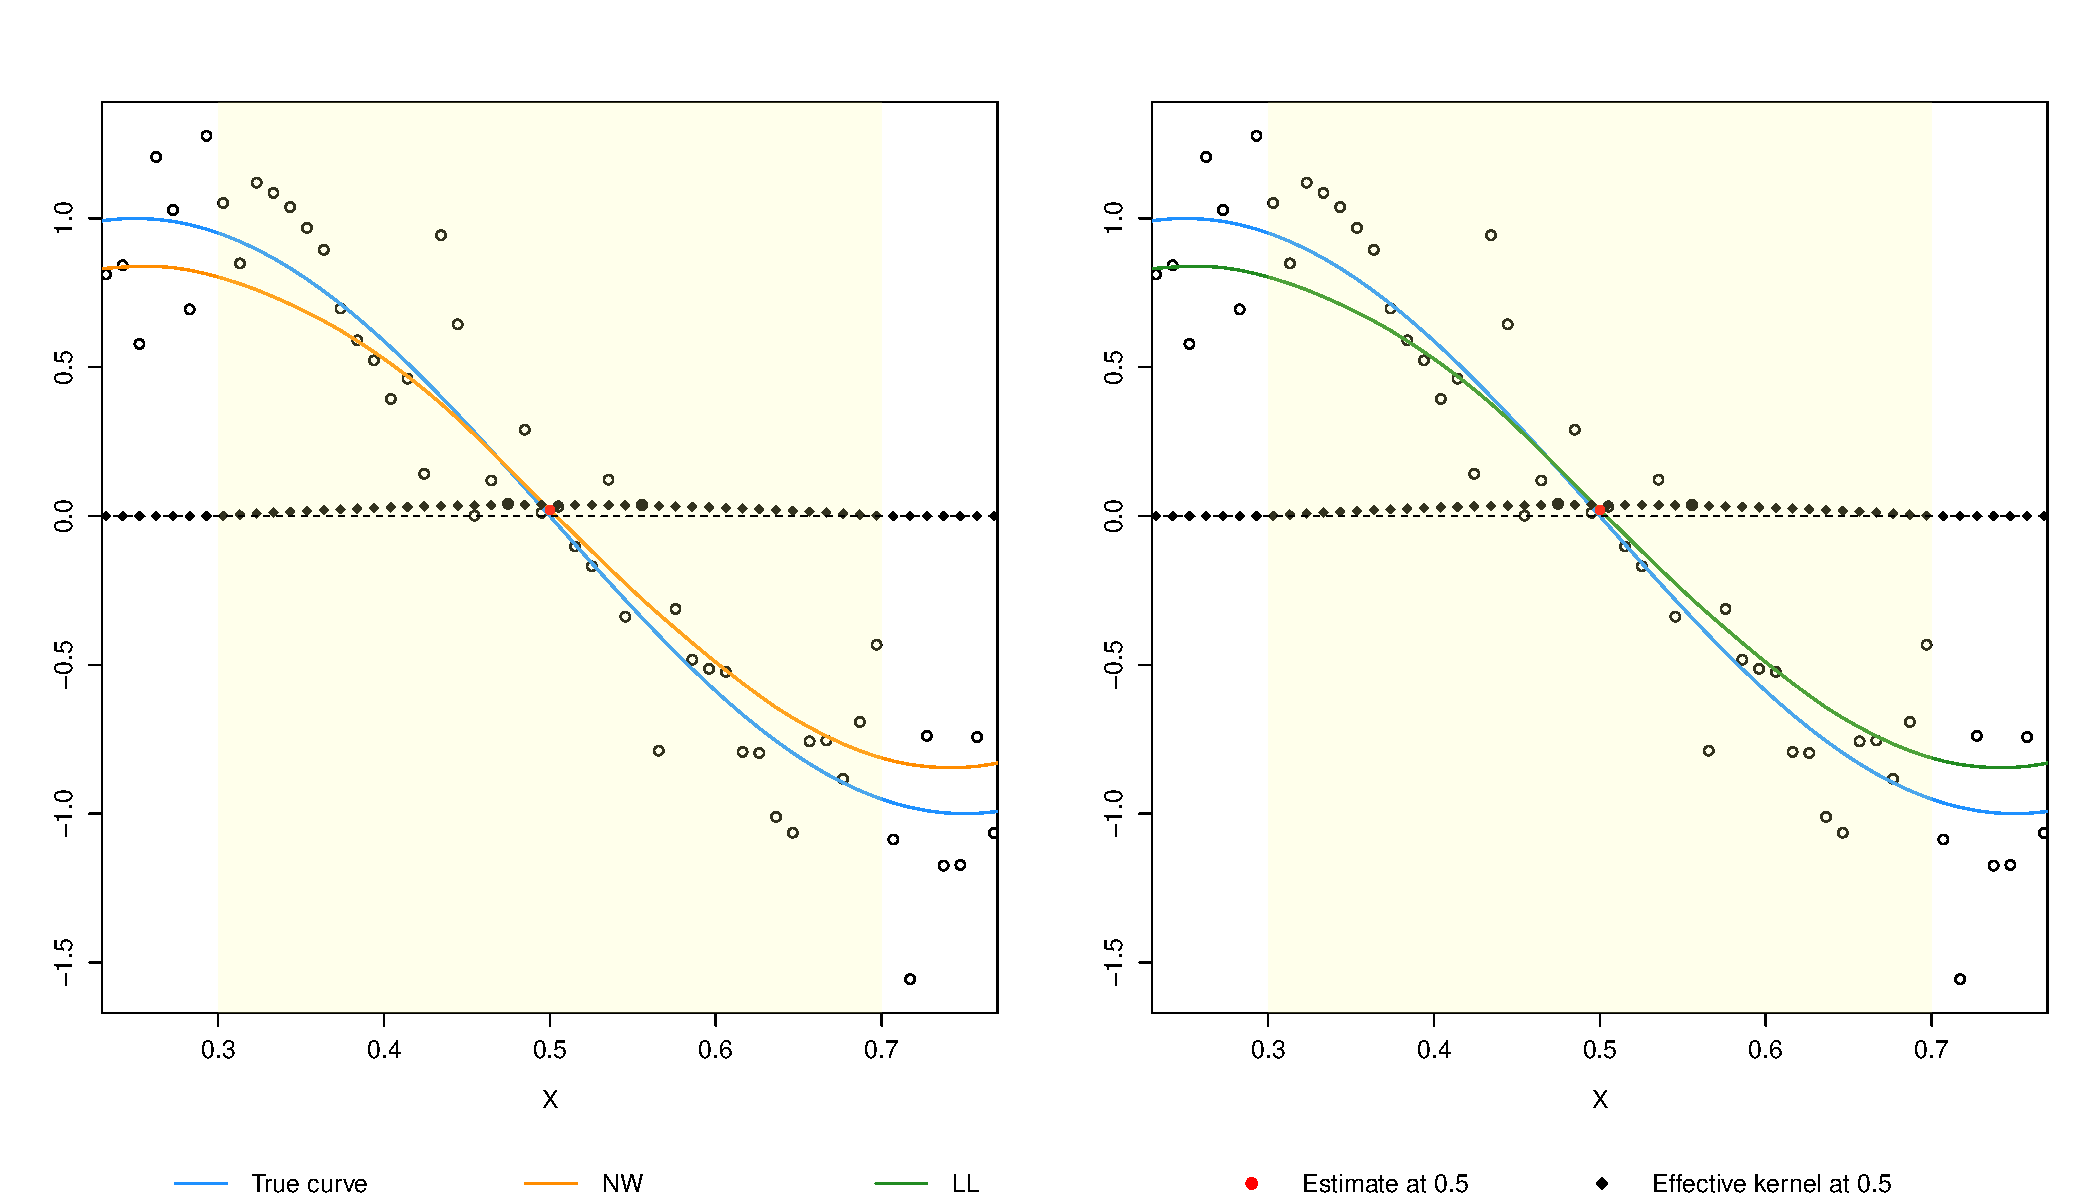
\includegraphics[trim=20 0 20 45, clip, width=\textwidth]{figure_03a.pdf}
		\caption{Effective kernel in the interior}
		\label{fig:effective_kernel_interior}
	\end{subfigure}
	
	\begin{subfigure}{0.75\textwidth}
		\centering
		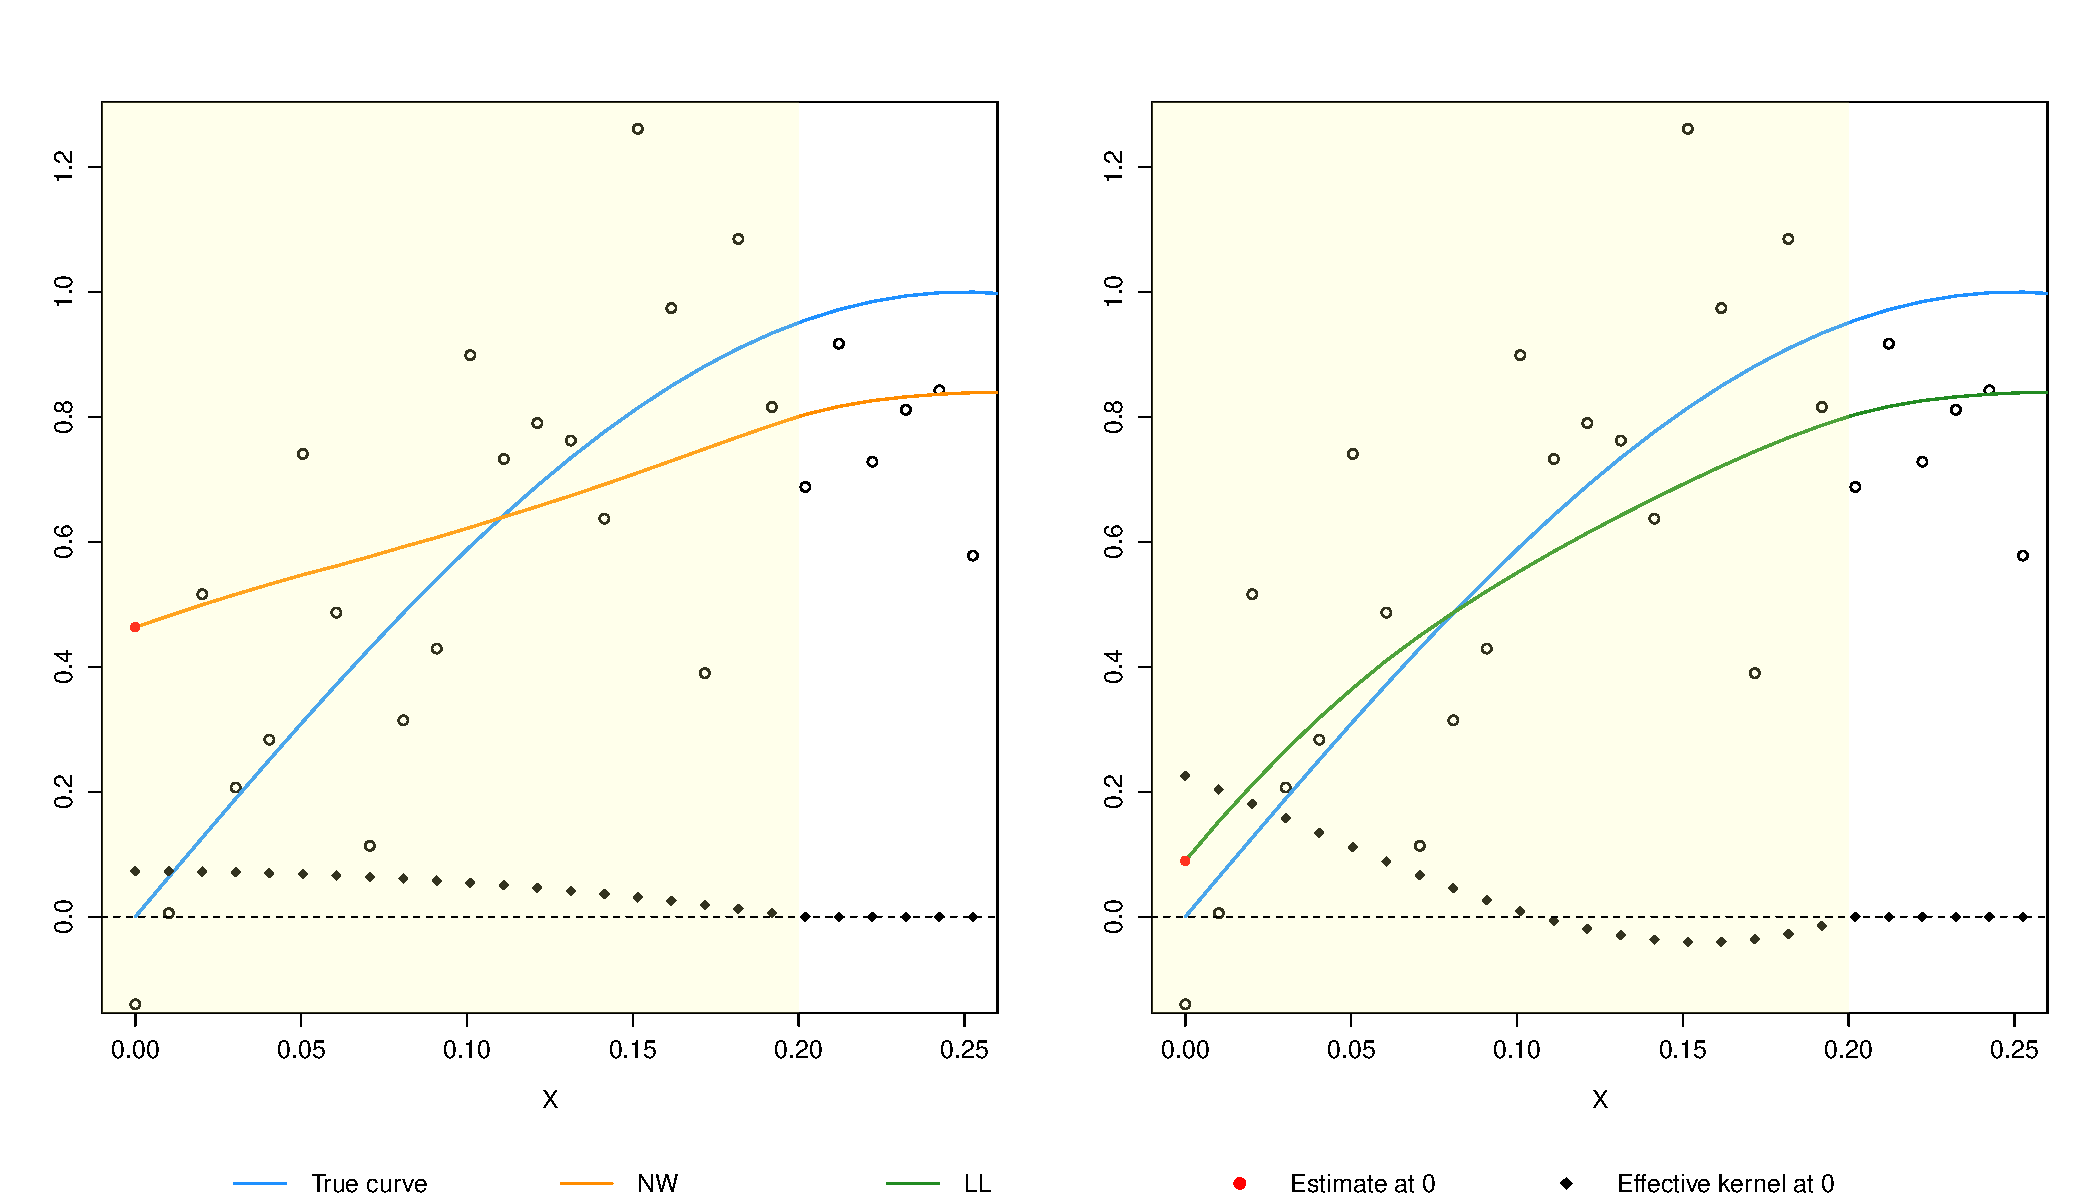
\includegraphics[trim=20 0 20 40, clip, width=\textwidth]{figure_03b.pdf}
		\caption{Effective kernel at the boundary}
		\label{fig:effective_kernel_boundary}
	\end{subfigure}
	\caption{Effective kernels for the Nadaraya-Watson estimator and the local linear estimator. The effective kernel is given by the filled squares.}
	\label{fig:effective_kernel}
\end{figure}

Figure~\ref{fig:effective_kernel_interior} shows the effective kernel for the Nadaraya-Watson and the local linear estimator, respectively, when estimating at the interior point $x = 0.5$.
The effective kernel is given by the black squares.
As these are literally the weights assigned to observations in the smoothing process, they sum up to one.
Only local data points in the yellow-shaded region receive positive weights, the more the closer $X_i$ is located to $x = 0.5$.
Overall, we do not see any difference between the two effective kernels.
The effectively assigned weights seem to be identical.

Next, we consider the estimation at the lower boundary $x = 0$.
This is presented in Figure~\ref{fig:effective_kernel_boundary}.
Once again, the large upward bias for the Nadaraya-Watson estimator is apparent.
Bias for the local linear estimator is much reduced.
For the Nadaraya-Watson estimator the effective kernel is just a rescaled version of the right side of the Epanechnikov kernel such that the added weights are one.
All weights in the estimation window are positive.
For local linear regression, in contrast, there are two effects visible leading to the improved boundary behavior.
First, $\hat{m}_{\LL}$ effectively assigns a much larger weight to observations in the immediate vicinity to $x = 0$.
Second, it puts a negative weight on the observations that are furthest away.
The negative weighting ensures that weights add to one and reverses the large bias observations far away from the boundary would contribute.
Figure~\ref{fig:effective_kernel_boundary} is a graphical illustration of Theorem~\ref{theorem_4}.
At boundary points the local linear estimator adapts automatically by deforming the effective kernel such that $\sum_{i = 1}^{n} w_i(x) (X_i - x) = 0$ holds.
The bias is removed to first order.